\renewcommand{\thechapter}{\arabic{chapter}}
\setcounter{chapter}{3}

\chapter{Données et méthodes cliniques}
\label{chap:chapter_4}
\chapterintro
Lors des précédents chapitres ont été présentés les trois domaines sollicités par ce travail. Ce nouveau chapitre se consacre à la présentation des données utilisées pour évaluer ces travaux et procède au recensement des méthodes cliniques sur les modalités concernées.\par

Dans un premier temps, la \textit{matière} utilisée afin de mener cette recherche est détaillée dans la \Cref{sec:clinical_data}. En effet, les expérimentations et résultats de ce manuscrit prennent appui sur une base de données initialement conçue pour la réalisation d'une étude clinique.  D’une part, cette étude clinique est décrite point par point en reprenant ses objectifs, les conditions d'inclusion permettant la constitution de la base de données, mais également les conclusions sur lesquelles ce travail s'appuie. D’autre part, une structuration de cette base de données est nécessaire ainsi que la mise à disposition d’une interface logicielle permettant l’accès à ses informations, présentés à la fin de cette section.\par

Dans un second temps, la \Cref{sec:clinical_methods} est dédiée à l’analyse de critères pertinents sur les trois modalités cliniques mises à disposition de ce travail. L'objectif de cette section est de comprendre les éléments importants recensés par les dermatologues lors d'un examen clinique.\par
\newpage

\section{Données de travail}
\label{sec:clinical_data}
Pour commencer, il est nécessaire de souligner que \textbf{cette base a reçu un agrément de la part du comité d'éthique du \acrfull{chuste}} pour son exploitation au sein de l'étude clinique mentionnée précédemment mais également pour ce travail universitaire (\textbf{numéro du comité d'examen institutionnel 672016/CHUSTE}). Par ailleurs, cette étude \textbf{est conforme aux recommandations de la déclaration de Helsinky}.\par

Par cette section, divers aspects de ces données de travail sont présentés. Dans un premier temps, une présentation de sa constitution et des données recueillies est amenée par la \Cref{sec:dataset_introduction}. Puis dans un second temps, les aspects liés à son organisation sont présentés dans la \Cref{sec:dataset_organisation}. Pour finir, cette section s'achève par la description de l'interface logicielle permettant l'interaction avec ces données dans la \Cref{sec:dataset_api}.\par

\subsection{Présentation des données}
\label{sec:dataset_introduction}
Cette base de données compile diverses \textbf{lésions faciales} possédant les critères d'inclusions suivants~:
\begin{itemize}
    \item les images proviennent de patients inclus entre les \textbf{années 2011 et 2015}, dont les données ont exclusivement été acquises au \textbf{\gls{chuste}},
    \item les données sont disponibles pour chaque patient sous trois modalités d'image différentes que sont la \textbf{photographie clinique}, la \textbf{dermatoscopie} et la \textbf{\gls{mcr}},
    \item les lésions considérées dans cette base sont celles dont le diagnostic différentiel, c’est-à-dire par élimination méthodique des causes (voir \Cref{subsec:lentigo}), était \textbf{fortement controversé} et \textbf{supposé comme appartenant à un \gls{lm} ou \gls{lmm}}.
\end{itemize}\par

En termes de composition, la base regroupe 201 patients répartis entre 96 femmes et 105 hommes d'un âge moyen égal à 70 ans compris entre 29 et 97 ans comme présentés sur la \Cref{fig:statistics_age_sex}. Cette base comporte 223 lésions uniques avec pour diagnostic de référence l'histologie. Ainsi, sont mis à la disposition de ce travail~:
\begin{itemize}
    \item 115 \textbf{lésions malignes}, scindée en 92 \gls{lm} et 23 \gls{lmm},
    \item 108 \textbf{lésions bénignes}, dont 20 \gls{cbc}, 37 \gls{ls}, 23 \gls{ks}, 15 \gls{kap}, 8 nævus, 2 kératoses lichénoïde, 2 cicatrices et 1 maladie de Bowen pigmentée.
\end{itemize}\par

Les acquisitions sont réalisées par l'un des trois experts investigateurs de l'étude clinique~\cite{Cinotti2018}. \textbf{Tout cas de collisions de tumeurs au sein est exclu de cette étude}. D'une part, les données de dermatoscopie sont produites à l'aide d'une caméra \textit{PowerShot® G7}~\textsuperscript{\ref{footnote:device_powershot}} couplée au dispositif proposé par \textit{Fotofinder}~\textsuperscript{\ref{footnote:device_fotofinder}}. D'autre part, les données de \gls{mcr} sont produites à l'aide d'un \textit{VivaScope 3000®}~\textsuperscript{\ref{footnote:device_mavig}}. En revanche, aucune information liée à l'acquisition des données de photographie clinique n'a été mentionnée.\par

\begin{figure}[H]
    \centering
    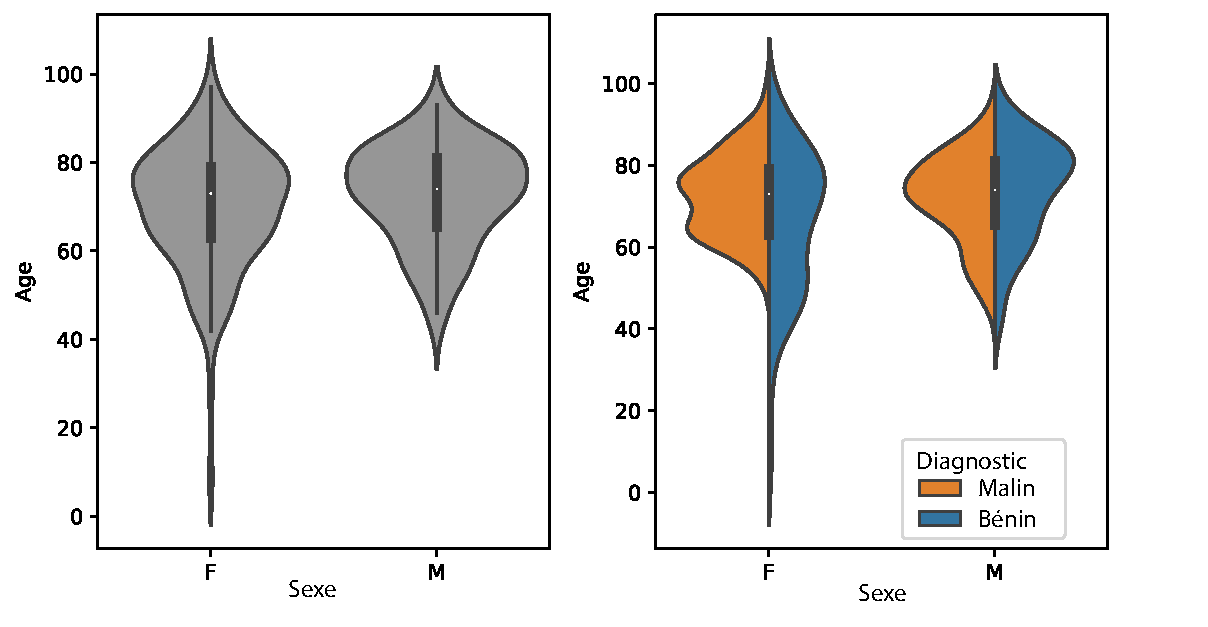
\includegraphics[width=\linewidth]{contents/chapter_4/resources/statistics_age_sex.pdf}
    \caption{À gauche, répartition en fonction de l'âge et du sexe. À droite, répartition entre l'âge et le sexe en tenant compte du diagnostic binaire.}
    \label{fig:statistics_age_sex}
\end{figure}\par

L'intérêt de ces trois modalités est grand dans le contexte de la dermatologie, puisqu'elles représentent le processus \textit{classique} de prise en charge clinique, de la modalité la moins onéreuse avec la \textbf{photographie clinique} mais également la moins précise, à des modalités plus onéreuses, également plus riches en information, avec la \textbf{\gls{mcr}}. Ainsi, chaque modalité permet au praticien de réduire, \textbf{si nécessaire}, la zone d'incertitude chez un patient souffrant d'une pathologie de la peau. Ce processus type de prise en charge peut être visualisé sur la \Cref{fig:scheme_devices_location}.\par

\begin{figure}[H]
    \centering
    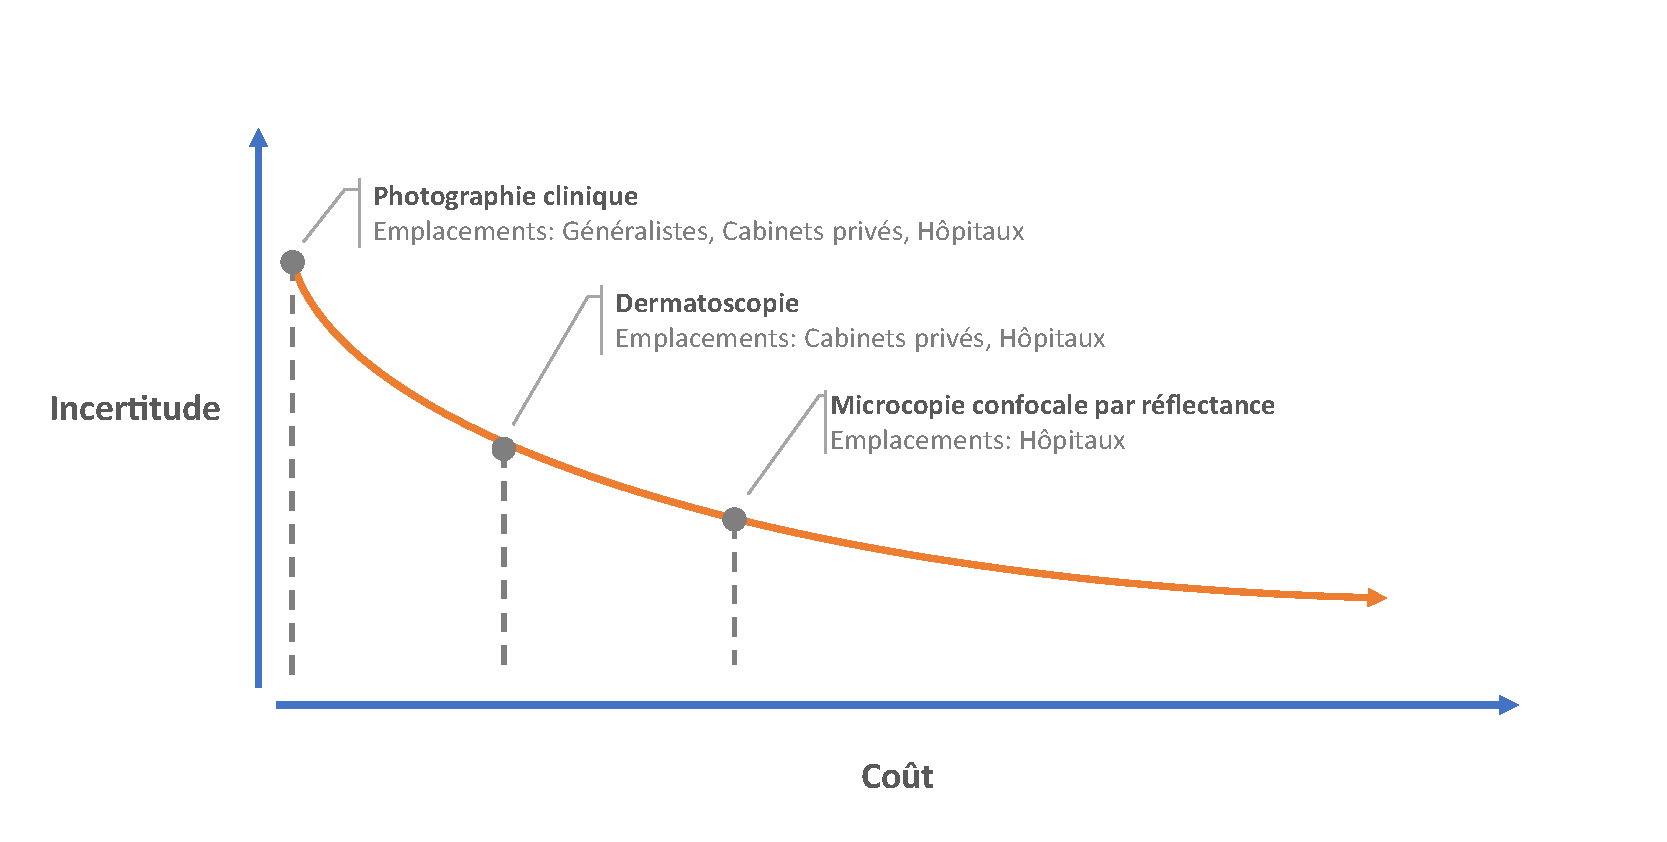
\includegraphics[width=\linewidth]{contents/chapter_4/resources/scheme_devices_location.pdf}
    \caption{Schéma de représentation du processus type de dermatologie, allant de la modalité la plus incertaine mais également la moins onéreuse, à la modalité la plus précise mais également la plus coûteuse.}
    \label{fig:scheme_devices_location}
\end{figure}\par

\addtocounter{footnote}{1}
\footnotetext[\thefootnote]{Source~:~Canon Powershot®, Canon, Tokyo, Japon. \label{footnote:device_powershot}}
\addtocounter{footnote}{1}
\footnotetext[\thefootnote]{Source~:~FotoFinder Systems GmbH, Bad Birnbach, Allemagne. \label{footnote:device_fotofinder}}
\addtocounter{footnote}{1}
\footnotetext[\thefootnote]{Source~:~Distribué en Europe par MAVIG GmbH, Munich, Allemagne. \label{footnote:device_mavig}}

Afin d'évaluer les performances de praticiens face à ces lésions, les investigateurs de l'étude de Cinotti et al. ont eu recours à 21 dermatologues détenant une expertise des modalités d'imagerie non-invasives. Ces experts sont répartis de manière homogène selon leurs compétences respectives pour chacun des dispositifs. Ainsi, le panel d'évaluation se décompose de la façon suivante~:
\begin{inlinerate}
    \item 6 experts sont soumis à l'ensemble des modalités,
    \item 15 experts sont soumis à l'évaluation de la photographie clinique et de la dermatoscopie (dont 9 uniquement dédiés a ces deux modalités),
    \item et 12 sont soumis à la \gls{mcr} (dont 6 uniquement dédiés à la \gls{mcr})~\cite{Cinotti2018}.
\end{inlinerate}
La répartition de ces experts est résumée en \Cref{fig:experts_evaluation}.\par

Ces experts ont évalué la gravité des lésions selon les termes \textbf{bénin} et \textbf{malin} pour chaque cas clinique présenté. Afin d'éviter un biais de la part des experts soumis à l'évaluation des trois modalités différentes, ceux-ci ont été sollicités sur trois journées séparées~:
\begin{inlinerate}
    \item une première journée d'évaluation ne comprenant que les images de photographie clinique et de dermatoscopie,
    \item une seconde journée d'évaluation ne comprenant que les images de \gls{mcr},
    \item et une dernière journée d'évaluation sur l'ensemble de la base d'images.
\end{inlinerate}
Par ailleurs, les cas cliniques ont été présentés dans un ordre différent entre chaque journée d'évaluation afin d'éviter des biais liés à l'activité précédente des experts.\par

\begin{figure}[H]
    \centering
    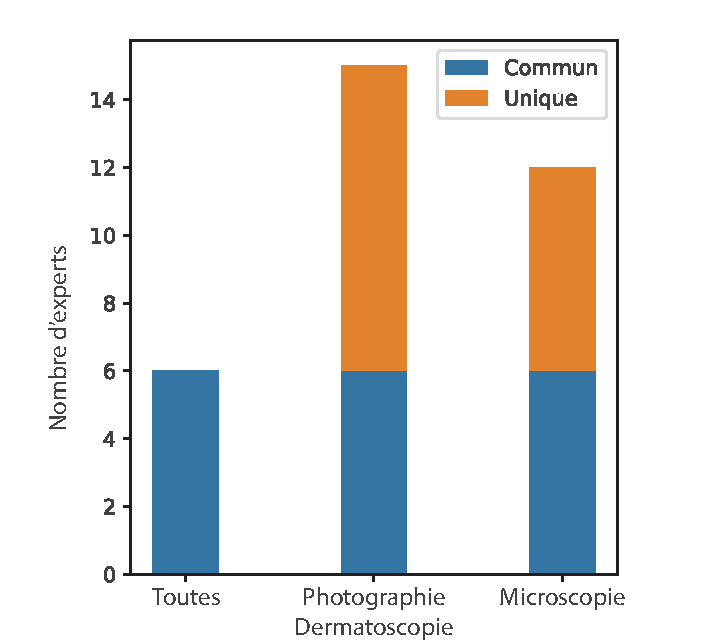
\includegraphics[width=0.75\linewidth]{contents/chapter_4/resources/experts_evaluation.pdf}
    \caption{Répartition du panel de 21 dermatologues sur l'évaluation des diverses modalités~\cite{Cinotti2018}.}
    \label{fig:experts_evaluation}
\end{figure}\par
\clearpage

\subsection{Structuration des données}
\label{sec:dataset_organisation}
Les données sensibles de cette base sont anonymisées afin de ne pas pouvoir ré-identifier les patients. Sa structure initiale peut être appréhendée sur la \Cref{fig:db_structure} - Haut, et se compose~:
\begin{itemize}
    \item d'un \textbf{tableau de lésions}, sous forme de fichier \gls{csv} et contenant~:
    \begin{itemize}
        \item \textbf{en colonne}, les diverses informations relatives au patient, soit \textit{l'âge, le sexe, la zone, son diagnostic binaire issu de l'histologie (malin ou bénin) et diagnostic précis},
        \item \textbf{en ligne}, les divers enregistrements liés à chaque lésion respectant les champs précisés en colonne.
    \end{itemize}
    \item d'un \textbf{répertoire d'images} comprenant les divers cas cliniques recensés dans l'étude sous divers formats d'image.
\end{itemize}\par

Afin d'exploiter au mieux cette base, quelques modifications sont apportées. D'une part, la diversité des formats images est un frein quant à la gestion de ces données, ainsi \textbf{un format matriciel sans perte de type bitmap} est adopté. D'autre part, la structure de la base dans l'état ne permet pas l'utilisation d'annotations au niveau des images ou des niveaux supplémentaires. Afin de rendre cet aspect plus dynamique, une structure reprenant les données de manière imbriquée est choisie. La racine de cette nouvelle structure reprend le tableau des lésions initial, dont chaque ligne est associée à une unique lésion. Ce procédé est ainsi répété de manière récursive, chaque dossier de lésion se compose lui-même de tableaux d'annotations propres au type d'annotations stockées. Par ailleurs, certains apports d'informations ont été réalisés pour permettre un bon déroulement de la suite de ce travail, tel que l'appartenance à un patient afin de ne pas proposer des données d'un même patient lors de l'entraînement et du test. Cette nouvelle structure est synthétisée sur la \Cref{fig:db_structure} - Bas.\par

\begin{figure}[H]
    \centering
    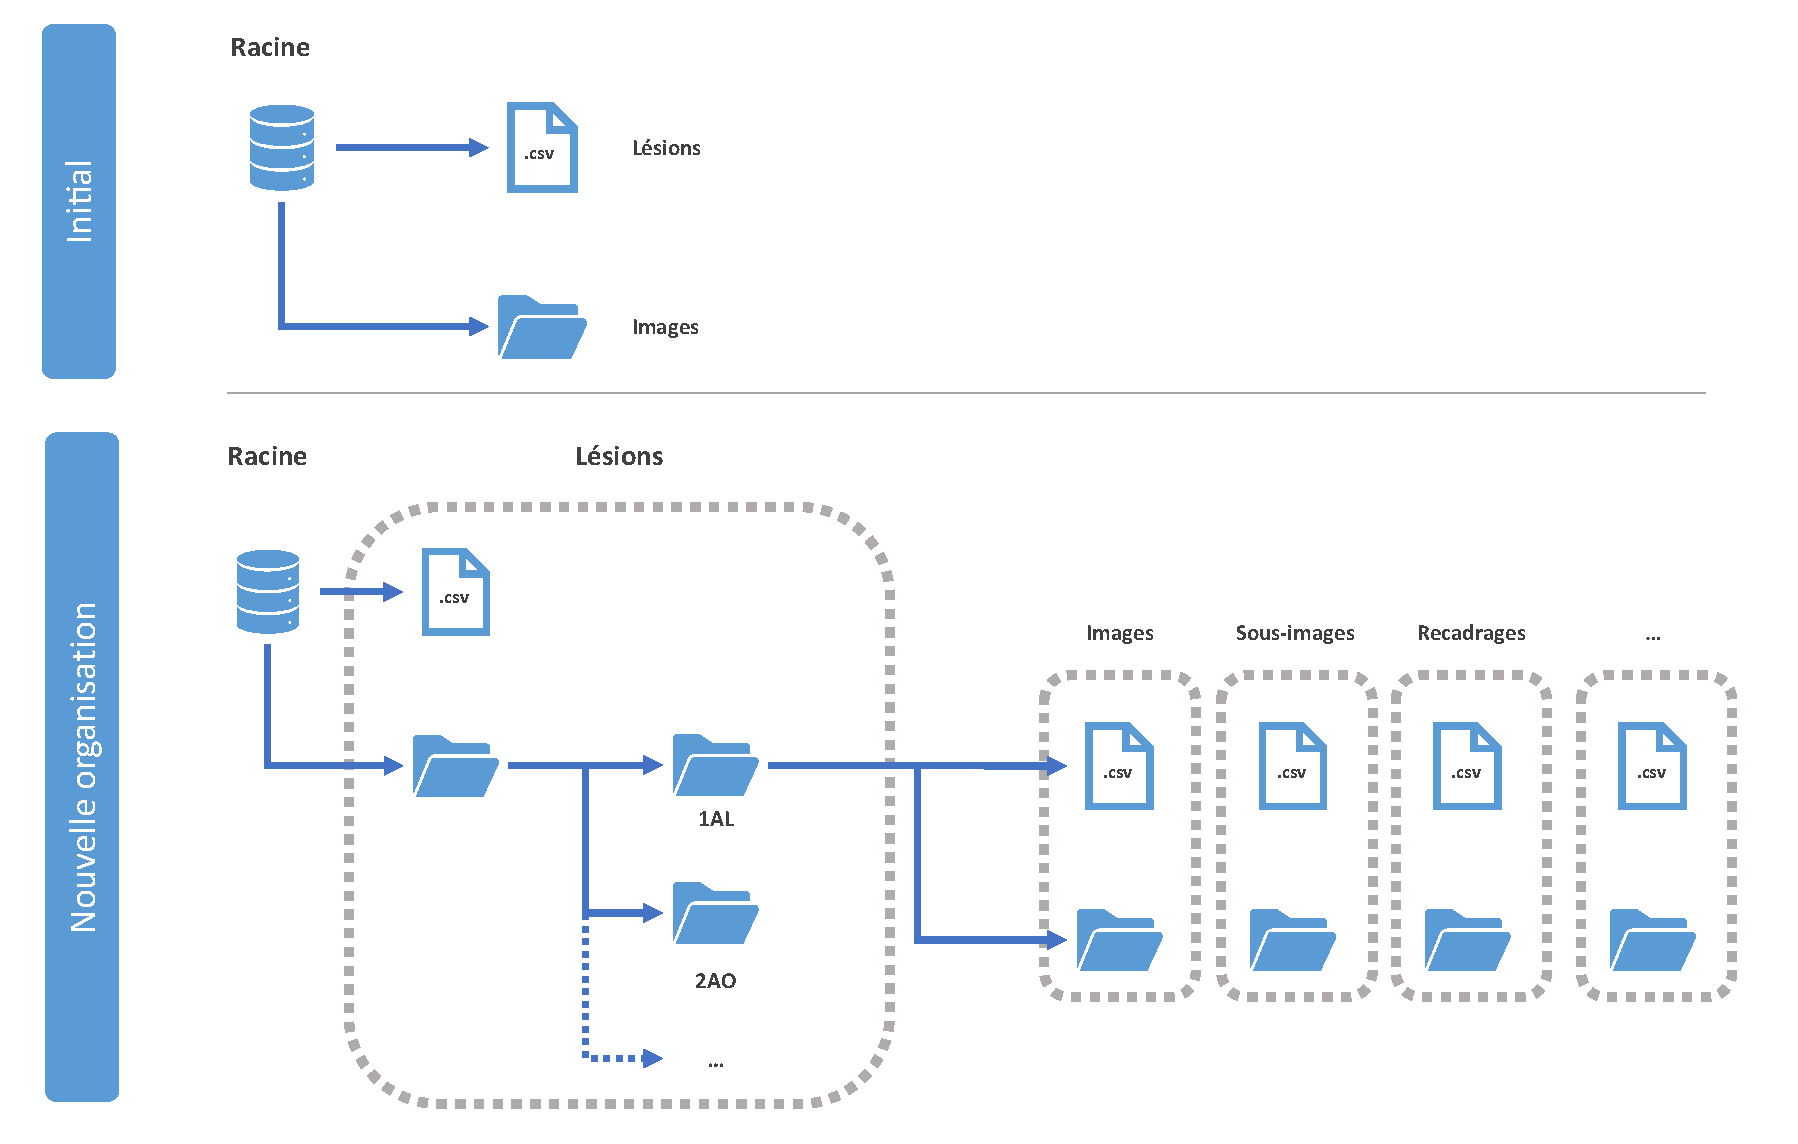
\includegraphics[width=0.9\linewidth]{contents/chapter_4/resources/scheme_data_structure.pdf}
    \caption{Schéma organisationnel de la base de données. En haut, la base initiale~;~En bas, la base restructurée afin de supporter de nouvelles annotations.}
    \label{fig:db_structure}
\end{figure}\par
\clearpage

\subsection{Interface logicielle}
\label{sec:dataset_api}
Malgré l'état actuel de la base de données, celui-ci ne permet pas son exploitation en l'état. Ainsi, un second aspect de la gestion de cette base de données a consisté à mettre en oeuvre une interface logicielle permettant d'accéder à celles-ci.\par

Les données de cette base au format image représente un volume non négligeable impossible à charger en mémoire vive avec la capacité à disposition de ce travail. Afin de ne pas excéder cette capacité, les données images sont chargées et maintenues en mémoire sous forme d'emplacement sur le disque dur jusqu'à leur utilisation définitive. Diverses méthodes d'accès à ces données sont mises à disposition, dont~:
\begin{itemize}
    \item une méthode \textit{get\_images()} avec pour objectif de retourner une structure de données sous forme de table contenant les méta-données et références aux images.
    \item une méthode \textit{get\_sliding\_window()} avec pour objectif de retourner une structure de données sous forme de table contenant les méta-données et références pré-extraites par balayage d'une fenêtre glissante \textit{en zone temporaire}.
    \item une méthode \textit{get\_multiple\_resolution()} avec pour objectif de retourner une structure de données sous forme de table contenant les méta-données et références pré-extraites par redimensionnement des images  \textit{en zone temporaire}.
\end{itemize} Chacune de ces méthodes met à disposition des arguments permettant de choisir d'une part la modalité ou encore le type d'annotations désiré et d'autre part des paramètres complémentaires liés au type d'extraction pour les principes de \textit{fenêtre glissante} et de \textit{résolutions multiples}. Cette interface logicielle mise à disposition peut être visualisée sur la \Cref{fig:schema_database_api}. Par ailleurs, les structures de données renvoyées par ces méthodes sont générées à l'aide de la librairie \textit{Pandas}~\cite{Pandas2020}.\par 

\begin{figure}[H]
    \centering
    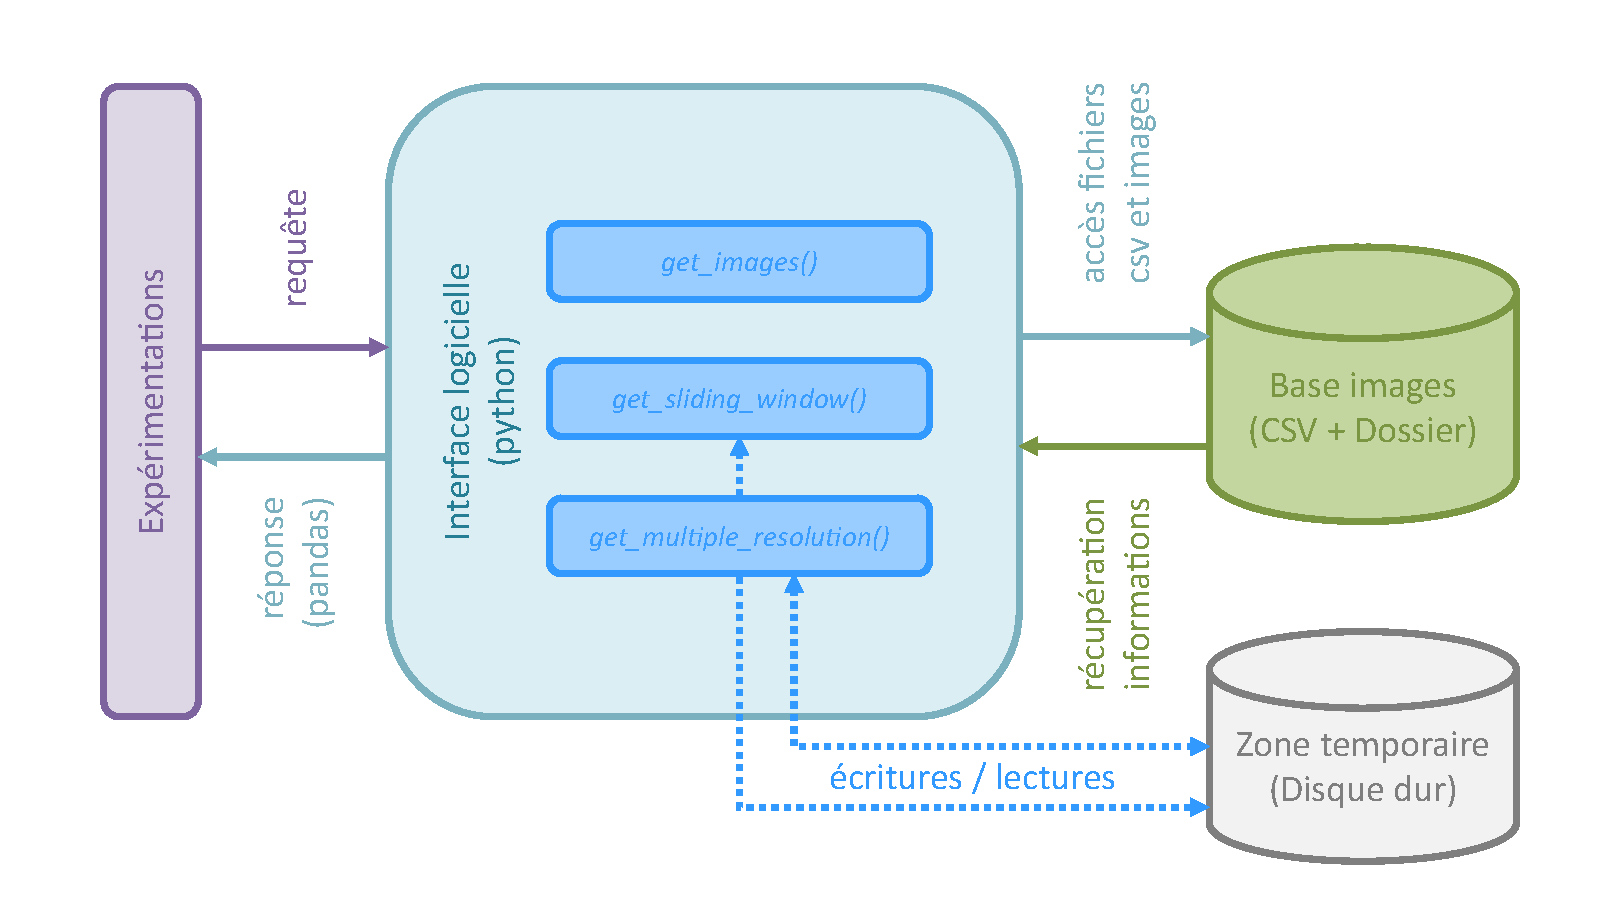
\includegraphics[width=\linewidth]{contents/chapter_4/resources/schema_database_api.pdf}
    \caption{Schéma de représentation de l'interface logicielle mise en place pour permettre les divers accès à la base mise à disposition. Par cette interface, trois méthodes sont mises à disposition des expérimentations qui suivent.}
    \label{fig:schema_database_api}
\end{figure}\par
\clearpage

\section{Méthodes clinique}
\label{sec:clinical_methods}
Pour permettre l'identification de pathologies en dermatologie plus routinière, la mise en avant de critères de diagnostic est une démarche clé mise en place pour rendre cette tâche plus efficace. Ces méthodes de mise en avant de critères ont démarré au milieu des années 1980 pour améliorer la prise en charge du mélanome, sous la forme~:
\begin{itemize}
    \item d'\textbf{acronyme}~:~l'idée est de proposer une méthode de diagnostic facile à mémoriser. Le précurseur de ces méthodes est le travail de Friedman, qui propose l'acronyme \textbf{ABCD} pour une observation à l'oeil nu de lésions pigmentées et est utilisable par de nombreuses personnes expertes ou non~\cite{Friedman1985}. Ainsi, cette première version insiste sur l'importance de quatre critères, dont~:~l'\textbf{A}symétrie, la \textbf{B}ordure (irrégularités), la \textbf{C}ouleur (variations) et le \textbf{D}iamètre (supérieur à 6mm). Cet acronyme s'est étendu à un cinquième critère d'\textbf{É}volution~\cite{Abbasi2004}.
    \item de \textbf{liste}~:~de critères positifs et négatifs, correspondant à des caractéristiques rédhibitoires ou non, et amenant à un score final. Ce score varie selon la pathologie considérée et permettra d'en déduire une décision à prendre. L'un des exemples dans le cadre de lésions pigmentées est celui de MacKie en 1986~\cite{mackie1986}. Ces critères ont été révisés et se destinent néanmoins à un public expert.
\end{itemize}\par

Ces démarches d'identification de critères clés pour parvenir à un diagnostic se sont progressivement étendues à une multitude de pathologies et de dispositifs d'analyse médicaux. Les pathologies de \gls{lm} et \gls{lmm} ne font ainsi pas exception à ce principe.\par

Dans certains travaux, l'utilisation de la dermatoscopie à permis une prise en charge précoce là ou la photographie clinique n'y parvient pas~\cite{Stante2005}. C'est donc naturellement que des critères sont recherchés sur la modalité de dermatoscopie, afin d'aider le praticien à diagnostiquer cette pathologie. Des caractéristiques propres aux pathologies de \gls{lm} sont ainsi mises en avant tels qu'une importante densité vasculaire, des structures rhomboïdes rouges, des motifs en forme de cibles ou encore un assombrissement lors de l'examen par dermatoscopie~\cite{Pralong2012}. Ces critères sont visualisables sur la \Cref{fig:example_dermoscopy_pattern}. Au moment de la rédaction de ce manuscrit, un travail de recherche reprend les critères précédemment cités et propose un ensemble de critères positifs et négatifs relatés dans la \Cref{tab:dermoscopy_algorithm_lentigo}. En déterminant un seuil de score d'une valeur de 1, ce travail parvient à détecter les pathologies de \gls{lm} avec une sensibilité de 0,95 et une spécificité de 0,75 sur une base de lésions contenant 42 \gls{lm} et 123 lésions bénignes~\cite{Ozbagcivan2019}.\par

\begin{table}[H]
    \centering
    \begin{tabular}{ll}
        \toprule
        Type de caractéristiques                        & Caractéristiques                                              \\\hline
        \multirow{5}{*}{Positives Mineures (+1 points)} & Assombrissement par observation avec dermatoscope             \\\cline{2-2}
                                                        & Présence de cercles gris                                      \\\cline{2-2}
                                                        & Motifs en forme de cible                                      \\\cline{2-2}
                                                        & Présence de rhomboïdes gris                                   \\\cline{2-2}
                                                        & Présence de points / globules gris ardoise                    \\\midrule
        \multirow{3}{*}{Négatives Mineures (-1 points)} & Présence de cercles blancs                                    \\\cline{2-2}
                                                        & Zones d'hyperkératose                                         \\\cline{2-2}
                                                        & Présence de rhomboïdes rouges                                 \\\bottomrule
    \end{tabular}
    \caption{Caractéristiques observables par dermatoscopie jugées pertinentes pour la détection du \gls{lm}~\cite{Ozbagcivan2019}.}
    \label{tab:dermoscopy_algorithm_lentigo}
\end{table}\par

\begin{figure}[H]
    \begin{center}
        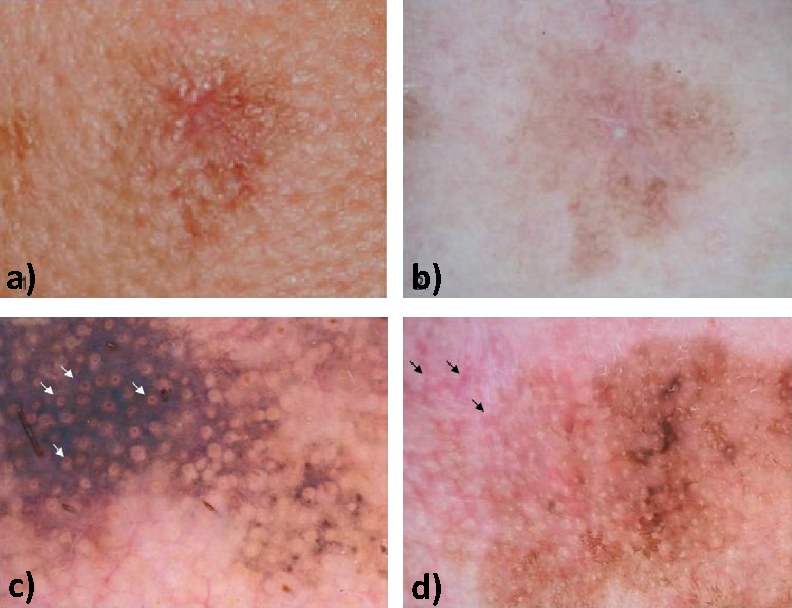
\includegraphics[width=\linewidth]{contents/chapter_4/resources/example_dermoscopy_pattern.pdf}
        \caption{Exemple de cas de données cliniques de dermatoscopie par Pralong et al.~\cite{Pralong2012}. En a) et b), exemple de phénomène d'assombrissement sur un cas de \gls{lm}~;~en c), exemple de motifs en forme de cible issue d'un \gls{lm}~;~en d), exemple de structure rhomboïdales rouges sur un cas de \gls{lmm}.}
        \label{fig:example_dermoscopy_pattern}
    \end{center} 
\end{figure}\par

La modalité de \gls{mcr} n'est pas exempte de ces démarches simplifiées, notamment pour le diagnostic du \gls{lm} avec les travaux de Pellacani et al. et de Guitera et al.~\cite{Pellacani2007, Guitera2010}. Ces deux travaux proposent sous forme de table de critères ceux jugés positifs et négatifs, dont la \Cref{tab:rcm_algorithm_lentigo} donne un aperçu de la production de ces articles. Leur étude comptabilise 81 cas de \gls{lm} et 203 lésions bénignes, sur lesquels une valeur de seuil de 2 a été jugé comme pertinente au regard de l'étude statistique menée. Celui-ci a permis de détecter avec 85~\% de sensibilité et 76~\% de spécificité les \gls{lm}.\par

\begin{table}[H]
\centering
    \begin{tabular}{ll}
        \toprule
        Type de caractéristiques                        & Caractéristiques                                              \\\hline
        \multirow{2}{*}{Positives Majeures (+2 points)} & Papilles à contour faiblement définis                         \\\cline{2-2}
                                                        & Cellules pagétoides rondes >\SI{20}{\micro\metre}             \\\midrule
        \multirow{3}{*}{Positives Mineures (+1 points)} & Présence de cellules atypiques dans la \gls{jde}              \\\cline{2-2}
                                                        & Combinaison de follicule / cellules atypique / pagétoide      \\\cline{2-2}
                                                        & Présence de cellules nucléées au sein de papilles             \\\midrule
        Négatives Mineures (-1 points)                  & Motif en alvéoles larges                                      \\\bottomrule
    \end{tabular}
    \caption{Caractéristiques observables par \gls{mcr} jugées pertinentes pour la détection du \gls{lm}~\cite{Guitera2010}.}
    \label{tab:rcm_algorithm_lentigo}
\end{table}\par
 
Ainsi, une caractéristique a été déterminée comme pertinente par leurs auteurs lorsque celle-ci s'exprimait de manière plus significative dans l'un des deux groupes pathologiques (\gls{lm} ou bénin). L'un de ces travaux~\cite{Guitera2010} procède à une analyse de ces caractéristiques par profondeur croissante de la peau, dont peuvent être cités les éléments majeurs suivants~:
\begin{itemize}
    \item au niveau de \textbf{l'épiderme}, les auteurs ont constaté que les pathologies de \gls{lm} comportent un désordre des cellules de l'épiderme (56~\% des lésions \gls{lm} contre 18~\% des lésions bénignes). Également, une infiltration pagétoïde a été reportée dans la plupart des cas de \gls{lm} (75~\% des lésions \gls{lm} contre 28~\% des lésions bénignes). En opposition, un épiderme homogène, caractérisé par des motifs en nid d'abeilles, a été constatés dans 92~\% des cas bénins. Ces éléments peuvent être observés sur la \Cref{fig:example_rcm_pattern_1}.
    \item au niveau de la \textbf{\gls{jde}}, les auteurs ont constaté que les papilles non démarquées étaient observées dans la majorité des \gls{lm} (68~\% \gls{lm} and in 17~\% des cas bénins). Ces éléments peuvent être observées sur la  \Cref{fig:example_rcm_pattern_2}.
    \item au niveau du \textbf{derme}, 15~\% des cas de \gls{lm} présentent des cellules nucléées larges contre 2~\% des lésions bénignes. Ces éléments peuvent être observées sur la \Cref{fig:example_rcm_pattern_3}.
\end{itemize}\par

Dans l'étude menée par Cinotti et al.~\cite{Cinotti2018}, les auteurs investigateurs ont demandé d'évaluer certaines caractéristiques récurrentes de la littérature, parmi lesquelles~:
\begin{itemize}
    \item la présence de grandes cellules pagétoïdes arrondies, présentes dans 37~\% des \gls{lm} et seulement 5~\% des pathologies bénignes,
    \item la présence de grandes cellules dendritiques dans l'épiderme, présentes dans 81~\% des \gls{lm} contre 13~\% des pathologies bénignes,
    \item la localisation au niveau des follicules pileux des cellules atypiques, dans 62~\% des \gls{lm} et seulement 7~\% des pathologies bénignes.
\end{itemize}\par

\begin{figure}[p]
    \begin{center}
        \includegraphics[width=\linewidth]{contents/chapter_4/resources/example_rcm_pattern_1.pdf}
        \caption{Exemples de cas de données cliniques \gls{mcr} en provenance de l'épiderme par Guitera et al.~\cite{Guitera2010}. En a) et b), exemples de motifs en nid d'abeilles (\textit{broadened honeycomb pattern}), respectivement d'une \gls{ks} et de peau normale~;~en c), exemples de motifs de pavés atypiques (\textit{atypical cobblestone pattern}) issus d'un \gls{lm}~;~en d), exemples de \textit{grandes cellules pagétoïdes} propres au \gls{lmm}. Repère~:~barre = \SI{50}{\micro\metre}.}
        \label{fig:example_rcm_pattern_1}
    \end{center} 
\end{figure}\par

\begin{figure}[p]
    \begin{center}
        \includegraphics[width=\linewidth]{contents/chapter_4/resources/example_rcm_pattern_2.pdf}
        \caption{Exemples de cas de données cliniques \gls{mcr} par Guitera et al.~\cite{Guitera2010}. En a) et au niveau de la flèche, exemple de papille à frontière non marqué (\textit{Nonedge papillae}) et de cellules atypiques d'un \gls{lm} acquise à la jonction \gls{jde}~;~En b), exemple de papilles à frontières marquées (\textit{Edge papillae}) d'une pathologie bénigne. En c), exemple de cellules atypiques au niveau de la \gls{jde} typique de \gls{lm}~;~En d), exemple de halo noir autour de cellules atypiques de l'épiderme issue d'un \gls{lm}. Repère~:~barre = \SI{50}{\micro\metre}.}
        \label{fig:example_rcm_pattern_2}
    \end{center} 
\end{figure}\par

\begin{figure}[H]
    \begin{center}
        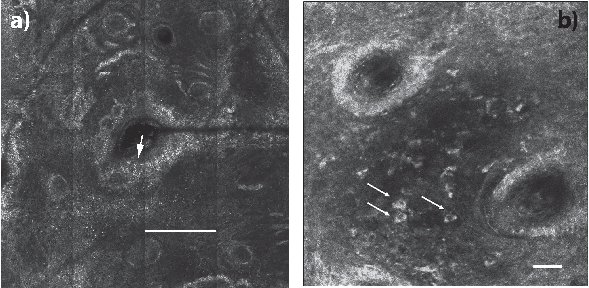
\includegraphics[width=\linewidth]{contents/chapter_4/resources/example_rcm_pattern_3.pdf}
        \caption{Exemples de cas de données cliniques \gls{mcr} par Guitera et al.~\cite{Guitera2010}. En a), exemple de cellules atypiques à proximité d'un follicule pileux au sein de la \gls{jde} sur un \gls{lm}~;~En b), exemple de cellules nucléées du derme d'un \gls{lm}. Repère~:~barre = \SI{50}{\micro\metre}.}
        \label{fig:example_rcm_pattern_3}
    \end{center} 
\end{figure}\par

% \section{Démarches d'aide au diagnostic}
% \label{sec:cad_methods}
% \subsection{Photographie clinique}
% Il s’agit du premier type d’images pouvant être produit lors de la prise en charge d’un patient pour des raisons dermatologique. Cette modalité, qui pour rappel consiste en un cliché à l’aide de dispositifs standards (appareil photo, smartphone, etc…) est de grande importance puisqu’elle sert de première interface entre la dermatologie et le patient. Son intérêt est d’autant plus grand avec l’avènement des solutions mobiles.
% Néanmoins, si nous comparons quantitativement le nombre de travaux menés, ceux-ci sont moindres en comparaison du dermatoscope. En effet, outre la diversité de capteurs propres à cette modalité, de nombreux éléments parasites peuvent altérer leur traitement de manière automatisée. Nous pouvons souligner la non constance des espaces de couleurs, l’inhomogénéité de l’éclairage, des aspects de réflectance présents et autre altérations telles que les poils. 
% Parmi ces rares travaux, nous pouvons citer dans des approches d’apprentissage standard, le travail menée par l’équipe de Giotis propre au mélanome [68]. Ce travail base son étude sur un premier traitement permettant la segmentation de la lésion, puis l’extraction de caractéristiques de couleurs et texture sur cette même région segmentée. Par ailleurs, l’auteur fait le choix d’un espace de couleur HSV plus cohérent avec la perception humaine. Des caractères supplémentaires sont également saisis par le médecin, en rapport avec le patient (âge, sexe, …) et l’aspect de la lésion.
% Au titre de ce travail, nous pouvons remarquer que l’un des aspects peux consister à modifier l’espace de couleur utilisé, dans le but de rendre les données moins dépendantes du capteur dont elles sont issues, l’une des caractéristiques type selon le critères ABCD pouvant être la couleur. Nous pouvons citer à titre d’exemple, l’utilisation de patches de référence afin de « calibrer » les capteurs [69].
% Certaines approches tentent d’apporter des solutions aux problématiques d’éclairage souvent présentes en photographie clinique. Ainsi ce second travail tente de répondre aux problèmes de réflectance dans l’image grâce aux travaux de Yang, puis apporte une correction de l’illumination afin d’homogénéiser cette dernière [70]. Ces corrections permettent d’optimiser le processus de segmentation et d’améliorer le retour d’information lié aux chromophores tels que l’hémoglobine et la mélanine.
% Notamment dans le cadre de lésions non pigmentaires, certains travaux laissent le travail de segmentation à l’opérateur et se concentrent sur les aspects de classification [71]. La plupart de ces travaux s’accordent sur l’extraction de caractéristiques de couleurs mais essentiellement de textures plus pertinentes, au travers de classifieurs traditionnels tels que SVM.
% D’autres approches plus poussées consistent à miser sur la masse de données disponible. C’est souvent sur cette vision que s’appuient des travaux basés sur les mécanismes d’apprentissage profond. L’une d’entre elles propose de reprendre un réseau pré entrainé sur des images génériques et donc composés de filtres également génériques, et de spécifier par un nouvel entrainement la couche de classification, moins couteux en ressources. Cette prouesse a permis l’obtention de résultat probants soit 72.1~\% de précision globale sur une classification à 3 classes : bénin, malin et non néoplasique [26]. Ce score a été obtenu à partir de données issues de photographie clinique mais également de dermatoscopie, composé de diverses pathologies visibles au travers de la Figure 51.

% \subsection{Dermatoscopie}
% Modalité la plus traitée dans le domaine de l’imagerie de la peau, le dermatoscope est 	aujourd’hui la modalité en vogue. En effet, la qualité de l’information fournie et sa faible altération par l’environnement en font une modalité fiable.  
 
% Figure 53 : Processus global de traitement des données.
% Afin de diminuer ces contraintes, il peut être envisagé d’utiliser les connaissances déjà acquises dans des domaines similaires par un transfert de connaissances . Le premier article [26] tente d’apporter une solution à notre problème à partir d’une architecture GoogleNet Inception v3 CNN  au préalable entrainée à l’aide d’une base contenant plus d’un million d’images lors d’un défi de 2014 intitulé « ImageNet Large Scale Visual Recognition Challenge». La  Figure 53 reprend le processus de bout à bout utilisé pour entreprendre la classification des lésions à grande échelle sur plus de 100 000 images. La classification des données selon l’arbre fourni en Figure 51, a permis d’obtenir les résultats suivants :
% - un premier degré de classification sur 3 classes, pour une précision de 72%. 
% - un second degré de classification sur 9 classes, pour une précision de 55%.

% \subsection{Microscopie confocale par réflectance}
% La microscopie confocale est une modalité qui semble s’inscrire dans une démarche de complémentarité vis-à-vis des examen de dermoscopie de routine [72]. Ainsi, elle permet dans un diagnostic mené par un humain, de rendre celui-ci plus spécifique. Pourtant, dans le domaine de l’aide au diagnostic automatique, des modalités les moins développées comparé à la dermoscopie. En effet, la littérature est plus pauvre sur cette thématique et n’offre qu’un développement assez succinct des pathologies de la peau avec essentiellement des cas de lésions mélanocytaires [73] et de lentigo [74], [75].
% Ces principales recherches peuvent être synthétisées sous le schéma classique de classification en 3 temps : Prétraitement, Extraction de caractéristiques et Classification (Figure 55). En effet, nous retrouvons ainsi lors de l’étape de pré traitement, un retrait du bruit parasite aléatoire. L’une des propositions en ce sens, est l’utilisation d’un filtre Gaussien passe bas, retirant les zones à forte énergie, c’est-à-dire à fort contraste dans une image. Ce même article fait référence à une égalisation d’histogramme afin d’homogénéiser les données avant traitements [76]. S’ensuit une étape d’extraction de caractéristiques pertinentes basés sur une représentation de la texture des images. Les éléments de littérature en notre possession s’axent essentiellement autour de l’utilisation d’ondelettes.  En effet, l’une d’entre elles part de l’utilisation d’une décomposition en ondelettes de Daubechies selon les axes horizontaux, verticaux et diagonaux, permettant de capturer les motifs présents dans nos données [74],[73]. Une seconde approche se base sur un descripteur de données (SURF) lui-même basé sur le principe d’ondelettes (Haar), et l’utilisation d’une approche par dictionnaire permettant l’obtention de caractéristiques sous forme de représentation par histogrammes [76]. Pour finir, une étape de classification est utilisée afin de déterminer le type de pathologie. La littérature propose l’utilisation de l’algorithme SVM ou de modèle d’arbre de classification [73], [74], [76].             
 
% Figure 55 : Synthétisation des processus de traitement proposées au travers de trois articles  [73], [74], [76].
% Enfin, l’un des travaux de recherche mené s’est basés sur une approche par apprentissage profond pour déterminer de manière automatique l’appartenance de l’image à l’une des couche de l’épiderme [77]. L’auteur utilise au préalable une approche par Texton combinée à un système de codebook afin d’obtenir un histogramme de fréquences [78] représentatif de chacune des couches

%~\cite{Wiltgen2008}
%~\cite{Halimi2017a}



